%
% variation1.tex
%
% (c) 2024 Prof Dr Andreas Müller
%
\begin{figure}
\centering
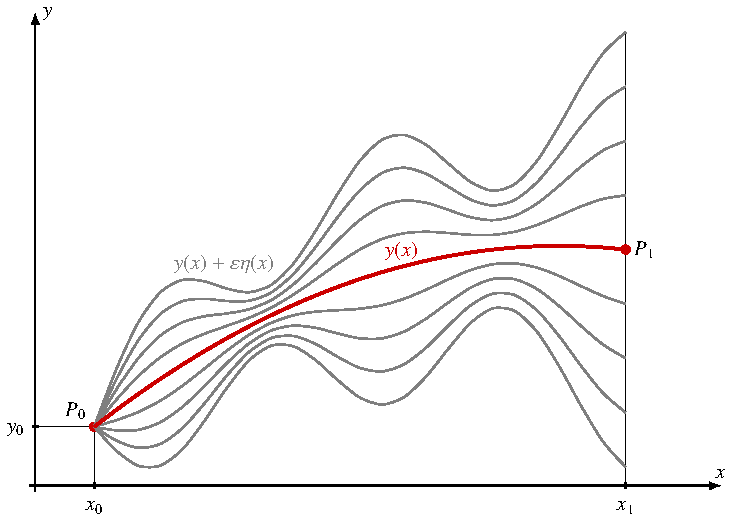
\includegraphics{chapters/020-variation/images/variation1.pdf}
\caption{Variation einer Funktion $y(x)$ durch Addition eines Vielfachen
$\varepsilon\eta(x)$ einer Funktion $\eta(x)$, die nur am linken Endpunkt
des Definitionsintervalls $[x_0,x_1]$ verschwindet: $\eta(x_0)=0$.
Das rechte Ende ist frei und liefert einen eigenen Beitrag zur ersten
Variation.
\label{buch:variation:fig:variation1}}
\end{figure}
